%%%%%%%%%%%%%%%%%%%%%%%%%%%%%%%%%%%%%%%%%%%%%
\section{Introduction}
\label{sec:intro}
%%%%%%%%%%%%%%%%%%%%%%%%%%%%%%%%%%%%%%%%%%%%%

The design and development of distributed systems is difficult and error prone.
Distributed systems are naturally concurrent, and suffer from network
partitions, partial failures and message reordering. Developers must reason
about all such corner cases when developing systems and protocols. To aid in
the development process specification languages such as
TLA+~\cite{Lamport:1993:HST:646874.709976}, Coq~\cite{WilcoxWPTWEA2015} and
ACL2~\cite{588534} have proven useful for designing verifiable protocols.
Recently Amazon has meade use of TLA+ to verify the most critical components of
AWS~\cite{Newcombe:2015:AWS:2749359.2699417} Unfortunately, these techniques
require a high level of skill to empoly, and ensuring that an implementation
does not diverge from it's verified specification is an unsolved problem. The
root of the problem is that real distributed systems are hard to test. They
must correctly handle all combinations of non-deterministic communication, and
local timeouts for all nodes in their systems. Reasoning about such an
exponential space of possibilities is difficult enough on simplified
specifications. In the current sate of verification, modestly sized sequential
programs can be verified for correctness, but the techniques simply do not
scale large systems, and especially not to large distributed systems. This
leads developers to use conventional techniques to test their systems.
Typically a distributed system test suit contains unit test for individual
components, integration tests for checking the correctness of separate
components. And stress tests, which involve placing the system under load, and
injecting failures. Of these tests unit, and integration, can typically be made
to easily pass under all conditions. Stress tests on the other hand can run for
long periods of time before bugs finally manifest themselves.  These failures
require the laborious manual inspection of large concurrently generated logs in
order to determine the sequence of events which triggered the bug. For these
reasons developers require tools for generating such bugs quickly in smaller
environments. 

The existing paradigms for generating these types of conditions fall into two
categories with some interesting projects in the middle. On one hand is fuzz
testing. Fuzz testers generate randomized input to cause a program to execute
many possible paths.  Fuzz testing is either blackbox or whitebox.  Blackbox
fuzz testing is similar to stress testing with the advantage that the input
which caused the system to fail can be more readily recovered. Modern blackbox
fuzzers use statistical techniques to generate inputs which extercise more
control flow paths than traditional random blackbox
testing~\cite{HouseholderProbabilityBasedParameter2012}. Whitebox fuzz testing
monitors aspects of a program such as control flow paths taken, and generates
new inputs to try and reach untested paths, a cutting edge example is
AFL~\cite{afl}. On the other end of the spectrum are some interesting attempts
at verification. Projects such as Modist~\cite{Yang:2009:MTM:1558977.1558992}
are black box distributed verification tools.  Modist instruments programs at
compile time in order to control all local timers and networking calls to the
operating system.  Modist then injects failures into the messaging and
non-deterministically fires timers. Modist enumerates through all inter
leavings of message failures, and non-deterministic timers to generate faults.
This process is slow, and has tight ties to bounded model checking where at any
$n+1$ non-deterministic event an unsafe state may be reached.  Whitebox
verification methods have also been developed recently. P\# is a verification
language which has demonstrated its efficacy by being integrated with systems
written in C\#~\cite{194442}. P\# allows users to write executable
specifications of their systems, and harnesses, similar to those used by SLAM
in device driver verification~\cite{Ball:2011:DSM:1965724.1965743}. Users than
test one component of their real system against the simplified specification.
Behind the scenes P\# verification engine enumerates the space of message inter
leavings and non-deterministic failures in order to cause the system to violate
either safety or liveness conditions. The downside to P\# is that developers
must maintain large ammounts of extra source code, in the form of
specifications in order to use P\#'s verification tool. In the centre of the
spectrum are mixtures of verification and fuzz testing.  Driller is a tool for
mixing symbolic execution and white box fuzz
testing~\cite{Stephens2016DrillerAF}.  Driller uses AFL to fuzz test programs.
When AFL is unable to explore new control flow paths, as is common which paths
which have a low probability of being executed randomly are present, digger
uses symbolic execution to determine what values will open up new control flow
compartments. The values are then fed back into AFL, and the fuzz tester can
continue to execute on new control flow paths. Digger has demonstrated it's
utility, but it is tailored for sequential programs which perform large
ammounts of file IO and not distributed systems.

Here we propose Obeah; a tool which uses SMT guided fuzz testing on distributed
systems written in Go. Conceptually Obeah is similar to Driller, but the
constraints of distributed systems demand an approach different from
conventional fuzz testing. Distributed systems cannot be fully tested by
manipulating file IO at a single entrance point. Insted they send and receive
messages from multipul connections using a variety of protocol. However,
reading a message from the network is a direct analog for reading in a file.
Our approach is to manipulate network messages in a similar way to fuzz
testing, while also using a control flow profile of the system to perform smart
manipulations on messages.  Obeah operates in two steps. First the source code
of a system is instrumented to report control flow, and mine control flow
information used during runtme analysis.  Second the system is tested under
normal operating conditions with a subset of the nodes in the system running
instrumented code. During execution the system is profiled. The profile
consists of a weighted control flow graph. Once a sufficient confidence measure
on the probability of control flow paths has been established Obeah attempts to
execute an low probability control flow path. To determine an low probability
path a bounded breadth first search is performed on the runtime CFG, and the
lowest probability path is selected as a candidate. During instrumentation each
branching statement is annotated with the set of conditions which must be
satisfied for its execution to occur. These conditionals include all parent
conditionals within their local functions.  Obeah passes the set of constraints
for the path to the Z3 constraint solver which determines if the constraints
are either unsat, or a set of variable values which satisfy the
constraint~\cite{deMoura2008}. If a satisfying assignment is found Obeah
directly modifies the values of variables which are set by incoming messages to
the values determined by the constraint solver.  This is processes is the same
as receiving a byzantine message. The values of the modified variables are
recorded and the system is allowed to progress. In the case where a failure
occurs, the set of variables altered by Obeah are reported to the developer. A
specific contribution of Obeah it's lack of symbolic execution. Adding latency
to a distributed system can cause timers to execute when they would not have
normally. Obeah forgoes the formality of using symbolic execution for the sake
of speed, and at the loss of precision.  However, it's techniques are often
enough to drive systems into failure states.

%eval

The rest of the paper as follows Section~\ref{sec:instrumentation} details
Obeah's instrumentation, and constraint learning process.
Section~\ref{sec:execution} covers Obeah's runtime environment, profiling, and
constraint generation. Section~\ref{sec:future} examines future work.

\begin{figure*}[t]
    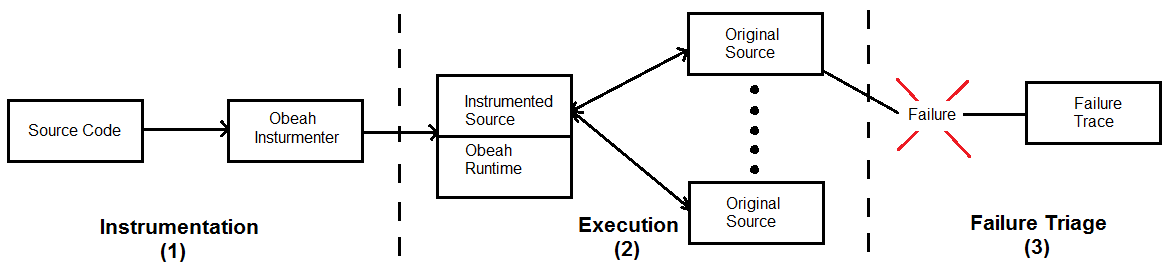
\includegraphics[width=\textwidth]{fig/obeah-system}%
    \caption{Overview of Obeahs workflow\label{fig:obeah-system}}%
\end{figure*}
